% Esta sección describe equipo y procedimiento de manera simple.
% Reemplaza con tu propio contenido cuando enseñes o evalúes.

% --- ESPACIADO GENERAL ---
\setstretch{1.2}                % Espaciado entre líneas
\setlength{\parskip}{6pt}       % Espacio entre párrafos

% --- ESPACIADO EN LISTAS ---
\setlist[itemize]{itemsep=6pt, topsep=6pt}

% --- ESPACIADO EN SUBTÍTULOS ---
\setlength{\parindent}{15pt}

\subsection{Actividad 1}

Para esta actividad, se requiere plantear el diseño un sistema embebido basado en un microcontrolador que gestione cinco tareas con diferentes requisitos temporales: la lectura de un sensor de alta velocidad (cada 10 ms), el control de un motor derivado de dicha lectura, el envío de telemetría vía serial (cada 100 ms), la actualización de una pantalla informativa y la atención inmediata de un botón de emergencia. El reto técnico consiste en garantizar que las tareas lentas (como la pantalla) no interfieran con las críticas (sensor y emergencia).

En la Figura~\ref{fig:problem_diagram} se observa el diagrama del problema descrito, junto con la estimación del tiempo total de ejecución del ciclo secuencial. La suma de las tareas da aproximadamente 75 ms por ciclo completo. Esto implica que, aunque el sensor debe leerse cada 10 ms, el ciclo completo tarda 75 ms, por lo que se pierden 6 de cada 7 lecturas. Asimismo, el botón de emergencia puede tardar hasta 75 ms en ser atendido, lo cual resulta inaceptable en un entorno industrial.

El reto técnico consiste en garantizar que las tareas lentas (como la pantalla) no interfieran con las críticas (sensor y emergencia).

\begin{figure}[htbp]
    \centering
    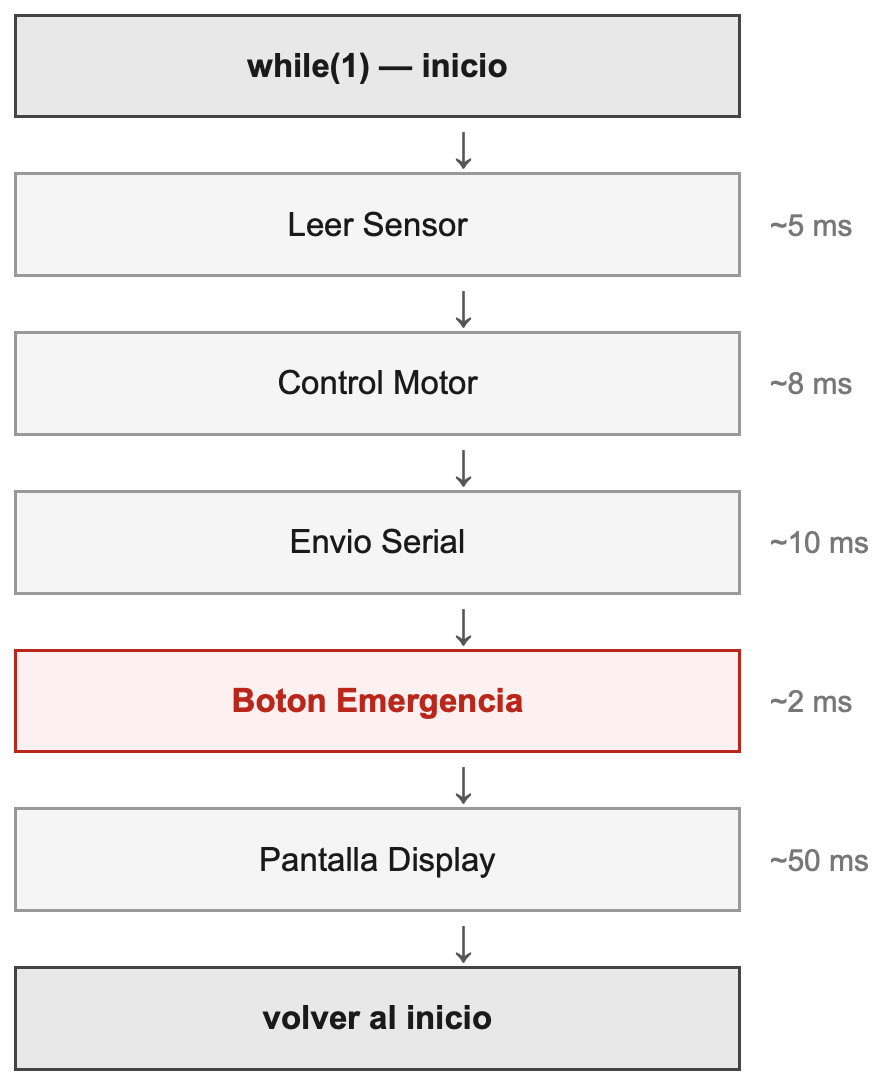
\includegraphics[width=0.9\linewidth]{images/problem_diagram.png}
    \caption{Diagrama del sistema secuencial con \texttt{while(1)} y tiempos acumulados por ciclo.}
    \label{fig:problem_diagram}
\end{figure}

\subsubsection{Discusión del caso}

En un entorno secuencial, todo el control reside en un bucle infinito donde el procesador ejecuta una instrucción tras otra. Para gestionar los tiempos, se suelen usar banderas o contadores de tiempo (como \texttt{millis()}). El código pregunta constantemente si es hora de leer el sensor o enviar datos, ejecutando las funciones solo cuando se cumple el tiempo establecido.

Sin embargo, el mayor riesgo de esto es el bloqueo por latencia. Si la tarea de "Actualizar pantalla" tarda 30 ms en completarse, el procesador quedará atrapado en esa función, impidiendo que el sensor se lea cada 10 ms. Esto genera una pérdida de datos y un control del motor errático. Además, el sistema se vuelve rígido, pues cualquier cambio en una tarea afecta el tiempo de todas las demás.

En esta tarea, la prioridad absoluta es el botón de emergencia, la cual es una medida de seguridad, por lo que no puede esperar a que un bucle termine su vuelta. Si el sistema está ocupado enviando un mensaje largo por el puerto serial y ocurre un accidente, un retraso de milisegundos en la detección del botón podría tener consecuencias catastróficas para el hardware o el operador \cite{verdugamonar_2025_controladores}.

Para asegurar el cumplimiento de los tiempos, es necesario transitar hacia una arquitectura orientada a eventos. Esto implica usar interrupciones para el botón de emergencia y los timers del sensor. Un RTOS facilitaría esto asignando prioridades, permitiendo que las tareas urgentes "expulsen" a las tareas lentas (como la pantalla) del CPU cuando sea necesario \cite{wirth_2022_superloop} \cite{verdugamonar_2025_controladores}.

\subsubsection{Solución propuesta}

La solución propuesta consiste en migrar de la arquitectura Super-loop a un RTOS (como FreeRTOS), donde cada tarea se ejecuta de forma independiente con su propio periodo y nivel de prioridad asignado por un Scheduler \cite{wirth_2022_superloop} \cite{verdugamonar_2025_controladores}. El botón de emergencia deja de ser una línea más dentro del bucle y se convierte en una interrupción hardware (ISR, del inglés, \textit{"Interrupt Service Routine"} o Rutina de Servicio de Interrupción), garantizando una respuesta en microsegundos sin importar qué esté haciendo el sistema \cite{wirth_2022_superloop}. El sensor se ejecuta como tarea periódica estricta cada 10 ms, el control del motor reacciona inmediatamente tras cada lectura, el envío serial corre cada 100 ms de forma independiente, y el display opera como tarea de fondo con la menor prioridad, de modo que sus 50 ms de ejecución nunca bloquean las tareas críticas. 

Así, el Scheduler se encarga de ceder y recuperar el CPU entre tareas según su urgencia, eliminando el problema central del Super-loop: que el tiempo de respuesta de cualquier evento dependa del tiempo de ciclo total del sistema.

\subsubsection{Respuesta Central: ¿Por qué no es suficiente un \texttt{while(1)}?}

Programar todo en un \texttt{while(1)} (conocido como arquitectura Super-loop) no es suficiente para sistemas complejos por tres razones críticas \cite{wirth_2022_superloop}.

En primer lugar, existe una falta de determinismo: el tiempo que tarda una vuelta completa del bucle depende de qué condiciones \texttt{if} se ejecutaron. Si la escritura en pantalla tarda 50\,ms, la lectura del sensor, que debe realizarse cada 10\,ms, se retrasará inevitablemente.

En segundo lugar, se produce una latencia inaceptable. Los eventos urgentes deben esperar a que el puntero del programa llegue a la línea donde se evalúa la condición correspondiente. En entornos de seguridad industrial, un retardo de 100\,ms puede ser suficiente para provocar un accidente.

Por último, se puede destacar que la arquitectura Super-loop es inescalable. A medida que se agregan funcionalidades, el código se vuelve frágil, por lo que modificar un simple \texttt{delay()} en una función puede comprometer el tiempo de respuesta de todo el sistema \cite{wirth_2022_superloop}.

En la Figura~\ref{fig:solution_diagram} se presenta el diagrama de la solución propuesta basada en un esquema con prioridades e interrupciones. El botón de emergencia se atiende mediante una interrupción hardware de máxima prioridad (ISR < 1 µs), garantizando respuesta inmediata. La lectura del sensor se ejecuta como tarea periódica cada 10 ms, seguida del control del motor como tarea reactiva. El envío serial se programa cada 100 ms, mientras que la actualización de la pantalla se ejecuta como tarea de fondo cuando el procesador está libre. Este enfoque asegura que las tareas críticas no sean bloqueadas por las de menor prioridad.

\begin{figure}[htbp]
    \centering
    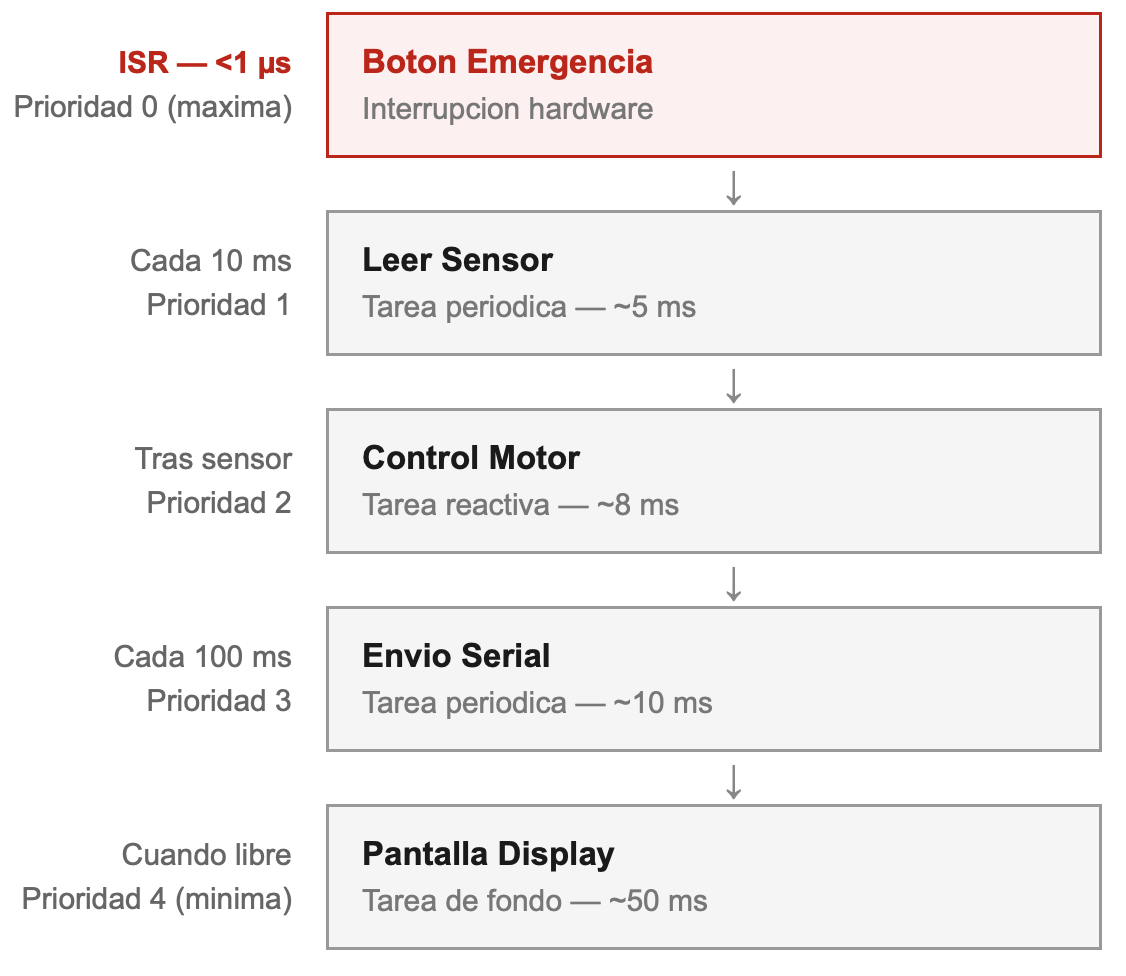
\includegraphics[width=0.9\linewidth]{images/solution_diagram.png}
    \caption{Arquitectura de solución basada en prioridades e interrupciones.}
    \label{fig:solution_diagram}
\end{figure}

\subsubsection{Material de consulta}

\paragraph{Interrupciones}

\begin{itemize}
    \item ¿Qué son?: Son mecanismos de hardware que permite al procesador suspender temporalmente la ejecución del programa principal para atender un evento urgente y específico \cite{sergio_2015_interrupciones}.
    
    \item ¿Cómo funcionan en un microcontrolador?: Actúa cuando ocurre un evento, el hardware completa la instrucción actual, guarda el estado del CPU en la pila (stack) y salta a una dirección de memoria fija llamada Vector de Interrupción, donde ejecuta la ISR (Rutina de Servicio de Interrupción). Al terminar, restaura el estado y vuelve al punto exacto donde se quedó \cite{sergio_2015_interrupciones}.
    
    \item ¿Qué problemas resuelven?: El Polling (preguntar constantemente). Sin interrupciones, el CPU pierde tiempo preguntando "¿ya presionaron el botón?" miles de veces por segundo \cite{sergio_2015_interrupciones}.

     \item ¿Qué riesgos implican?: Pueden causar corrupción de datos si no se manejan variables atómicas y, si son muy frecuentes, pueden provocar que el programa principal nunca se ejecute \cite{sergio_2015_interrupciones}.
     
\end{itemize}

\paragraph{Planificación y Scheduler}

\begin{itemize}
    \item ¿Qué es un scheduler?: Es el componente del núcleo (Kernel) encargado de decidir qué tarea (hilo) tiene el control del CPU en un momento dado \cite{ortega_2019_scheduler}.
    
    \item ¿Qué significa prioridad?: Es un valor numérico asignado a cada tarea. El Scheduler siempre favorecerá la ejecución de la tarea con mayor prioridad \cite{ortega_2019_scheduler}.
    
    \item ¿Qué es planificación preventiva y cooperativa?:
    
      \begin{itemize}

       \item Preventiva: El Scheduler puede "quitarle" el CPU a una tarea a la fuerza si aparece una de mayor prioridad. Es ideal para tiempo real.
       \item Cooperativa: Una tarea debe terminar o "ceder" voluntariamente el CPU para que otra pueda entrar. Si una tarea se queda en un bucle infinito, bloquea todo el sistema \cite{ortega_2019_scheduler}.
         
     \end{itemize}
  
\end{itemize}


\paragraph{Multitarea}

\begin{itemize}
    \item ¿Qué es concurrencia?: Es la capacidad del sistema para manejar múltiples tareas que parecen progresar simultáneamente, aunque en un solo núcleo se ejecuten una por una intercaladas \cite{sergio_2015_interrupciones} \cite{rivas_2012_multitarea}.
    
    \item Diferencia entre multitarea real y simulada:

       \begin{itemize}

       \item Real: Ocurre en procesadores de varios núcleos (Multi-core), donde cada núcleo ejecuta una tarea distinta físicamente al mismo tiempo.
       
       \item Simulada: Ocurre en microcontroladores de un solo núcleo mediante el Cambio de Contexto (Context Switching), alternando tareas tan rápido que el ojo humano no percibe la pausa \cite{rivas_2012_multitarea} \cite{verdugamonar_2025_controladores}.
         
       \end{itemize}
    
    \item Ejemplos en sistemas embebidos:

        \begin{itemize}

         \item Un sistema con RTOS como FreeRTOS donde:

             \begin{itemize}

             \item Una tarea maneja WiFi.
       
             \item Otra controla motores.

             \item Otra procesa datos de sensores \cite{verdugamonar_2025_controladores}.
         
            \end{itemize}
       
         \item En un ESP32 (doble núcleo):

               \begin{itemize}

               \item Núcleo 0 ejecuta la pila WiFi.
       
               \item Núcleo 1 ejecuta la lógica principal del usuario \cite{rivas_2012_multitarea}.
         
              \end{itemize}
         
        \end{itemize}
  
\end{itemize}

\paragraph{Sincronización}

\begin{itemize}
    \item ¿Qué es una condición de carrera?: Ocurre cuando dos o más tareas intentan modificar un recurso compartido (como una variable global) al mismo tiempo, dejando un resultado impredecible \cite{pez_2025_sincronizacion}.
    
    \item ¿Qué son semáforos y mutex?:

             \begin{itemize}

               \item Mutex: Abreviatura del inglés \textit{"mutual exclusion" }o exclusión mutua, es un "candado". Solo una tarea puede tener la llave para entrar a la sección crítica \cite{pez_2025_sincronizacion}.
       
               \item Semáforo: Es un "contador". Permite que un número limitado de tareas accedan a un recurso o sirve para señalizar entre tarea \cite{pez_2025_sincronizacion}.
              \end{itemize}

     \item ¿Qué es sección crítica?: Es la parte del código que accede a ese recurso compartido y que no debe ser interrumpida por ninguna otra tarea que use el mismo recurso \cite{sergio_2015_interrupciones} \cite{pez_2025_sincronizacion}.
     
\end{itemize}

% \begin{figure}[ht]          % Otra figura; [!b] sugiere colocación al pie de página
  % \centering
  % keepaspectratio asegura que no se deforme la relación de aspecto al escalar
  % width=0.9\linewidth establece el ancho relativo; se puede combinar con height=...
 %  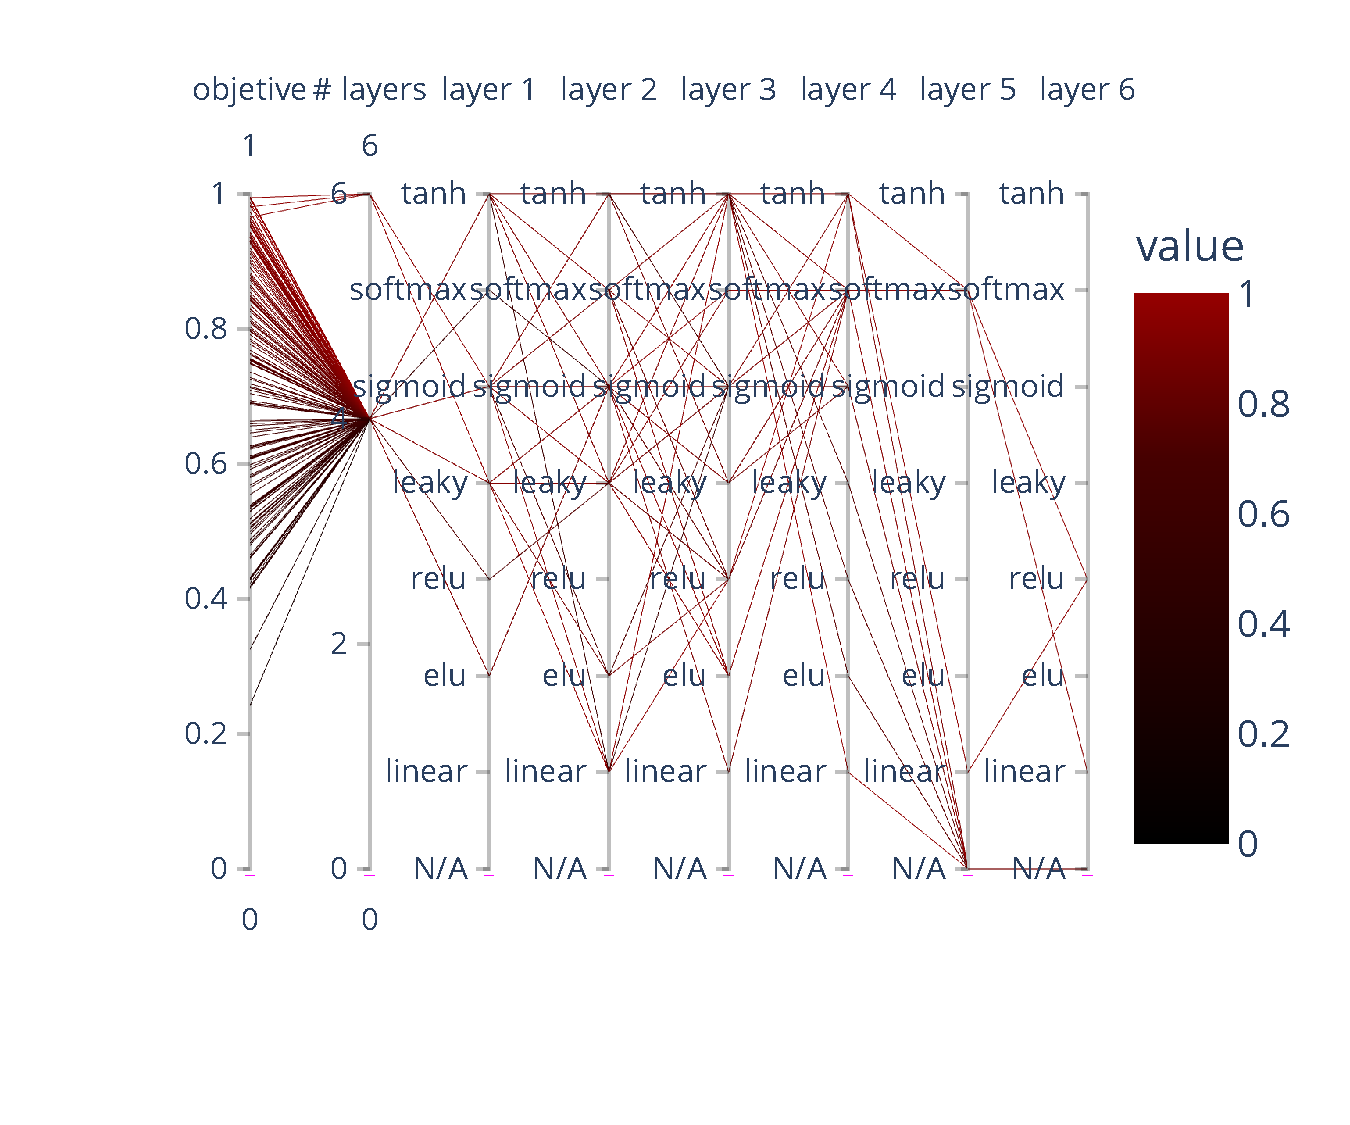
\includegraphics[keepaspectratio, width=0.9\linewidth]{images/act.pdf}
 %  \caption{Gráfico PGF de ejemplo (sustituible).}
  % \label{fig:ejemplo_pgf}   % Etiqueta para referencias cruzadas
%  \end{figure} 

% Fin de la sección de ejemplo.
